\chapter{电影推荐系统的设计与实现}
在前两章节中,本文主要介绍了实验性质的推荐算法模型,在本章节中,我们实现了长短期兴趣模型驱动的电影推荐原型系统MovieRec,
帮助用户快速发现自己喜爱的电影。MovieRec的推荐流程主要分为三个阶段,第一阶段中MovieRec读取所有用户的电影评分数据,
在长短期兴趣模型中生成每位用户和每部电影的特征表示;然后在第二阶段使用基于特征的协同过滤框架进行评分预测,
并将预测评分较高的电影整理成列表推荐给相关用户;最后第三阶段中,用户可以通过对推荐列表中的推荐项点赞或者差评进行反馈,
MovieRec会根据用户反馈进行动态调整,生成更好的推荐结果推送给用户。

\section{系统结构}
MovieRec可以分成三个阶段,如图\ref{fig:system}所示。

\begin{figure}[htbp]
\centering
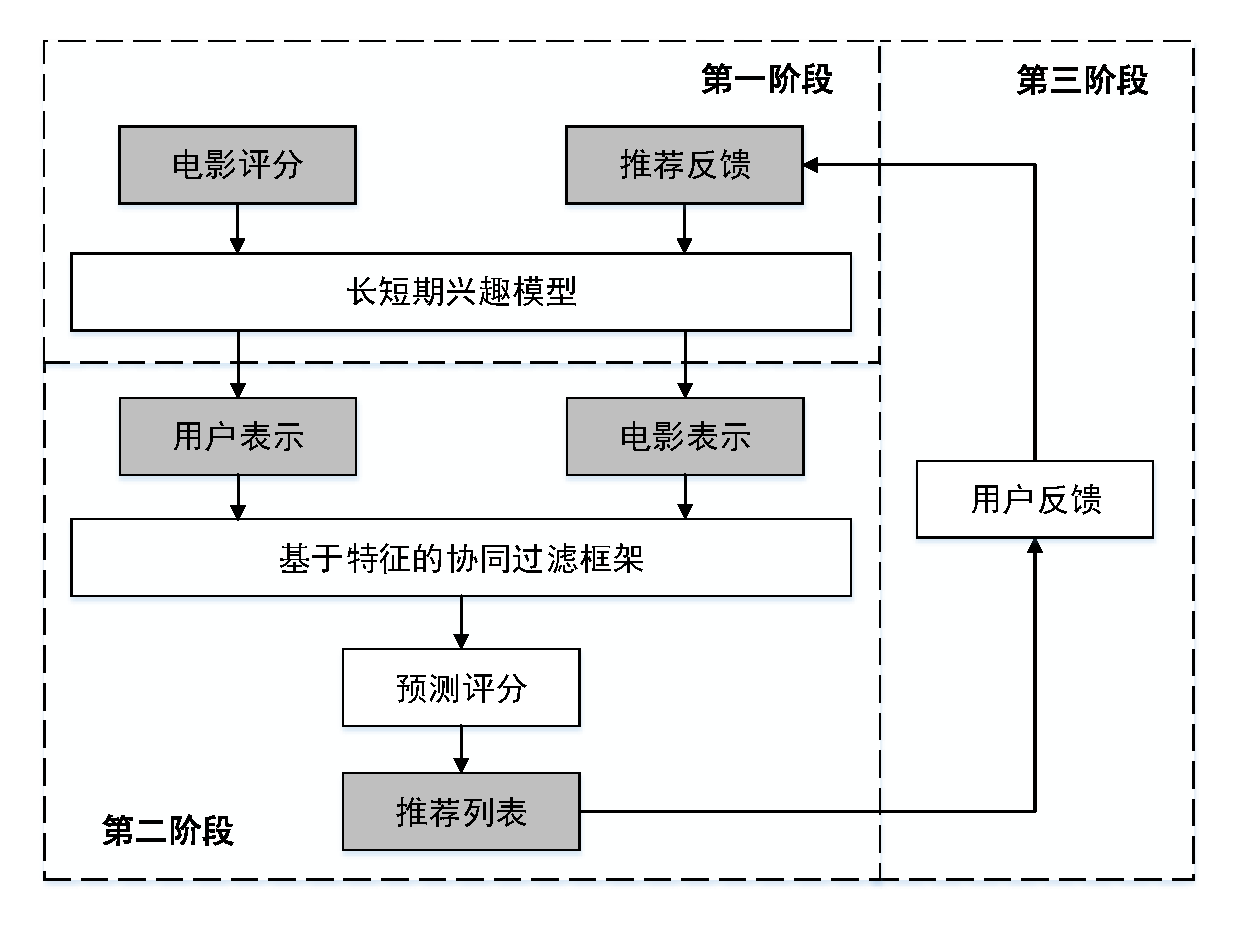
\includegraphics[scale=0.7]{images/system.pdf}
\caption{MovieRec系统结构图}
\label{fig:system}
\end{figure}

\section{第一阶段:用户电影特征表示生成}
在第一阶段中,MovieRec主要接受用户的电影评分数据和推荐反馈数据作为用户的行为信息,初始情况下,
我们会从公开数据集MovieLens-20M中预加载一些电影评分数据,毕竟一个没有任何评分数据的平台无法进行任何有效的推荐。
对于一个新注册的用户,在第一次登陆系统的时候,我们会随机提供一些热门的电影给用户进行评分,形成用户的初始行为数据,
用户可以在之后的使用过程中可以通过再次评分或者推荐反馈进行行为数据更新,帮助推荐系统为自己进行更好的推荐。

对于输入的电影评分数据和推荐反馈数据,MovieRec以用户为单元进行聚类,并且按照时间进行排序,形成了每个用户的观影时间线,
然后利用本文提出的长短期兴趣模型,生成对应的用户特征表示和电影特征表示,作为该阶段的输出内容。
特别地,MovieRec也提供了用户个人观影时间线界面,直观地向用户展示系统推荐的依据,该界面中,
用户还可以对比不同电影之间的相似度,查看自己观影兴趣的偏移。

\section{第二阶段:用户电影预测评分生成}
第二阶段中,利用基于特征的协同过滤框架,MovieRec把第一阶段输出的用户特征表示和电影特征表示作为输入,
把真实观察到的用户电影评分数据作为目标,利用已有的历史评分数据训练出一个评分预测的模型,从而对未知的电影评分进行预测,
并将其中预测分数较高的电影构成推荐列表推送给用户。同时,MovieLens还提供了基于其他推荐算法的推荐列表,
例如矩阵分解算法和因式分解机算法等,用户可以手动进行切换,对比观察不同推荐算法之间的区别和优劣性。

\section{第三阶段:用户动态反馈}
推荐给用户的电影列表中主要包含的电影信息有电影标题、电影类别和电影平均得分,用户可以通过点击操作进入到电影详情界面,
里面包含了最近一段时间的用户评分数据,以及用户给该电影打的标签。因为MovieRec中使用的是真实世界中的电影数据集,
所以还特别提供了其他三个电影推荐平台:MovieLens\footnote{https://movielens.org}、
IMDb\footnote{http://www.imdb.com}和TheMovieDb\footnote{https://www.themoviedb.org}中对应的电影详情界面的跳转链接,
在其中提供了更加丰富的电影信息,包括导演、男女主演、剧情简介、电影时长、海报剧照和社区数据等等。

为了让用户可以对推荐结果进行反馈,MovieRec在推荐列表中的每一项都提供了两项反馈操作,分别是正反馈``点赞''和
负反馈``差评'',用户可以通过这两个反馈表示自己对推荐结果的满意情况。具体实现中,
我们将``点赞''操作认为是用户给该项推荐结果进行了最高分的评分($5$分),
将``差评''操作认为是用户给该项推荐结果进行了最低分的评分($1$分),从而加入到第一阶段的用户电影特征表示的更新过程中。

\section{系统展示}
本章节中,我们将展示MovieRec电影推荐系统中的各个模块,分别是电影推荐界面、个人观影时间线界面和电影详情界面。

\begin{figure}[htbp]
\centering
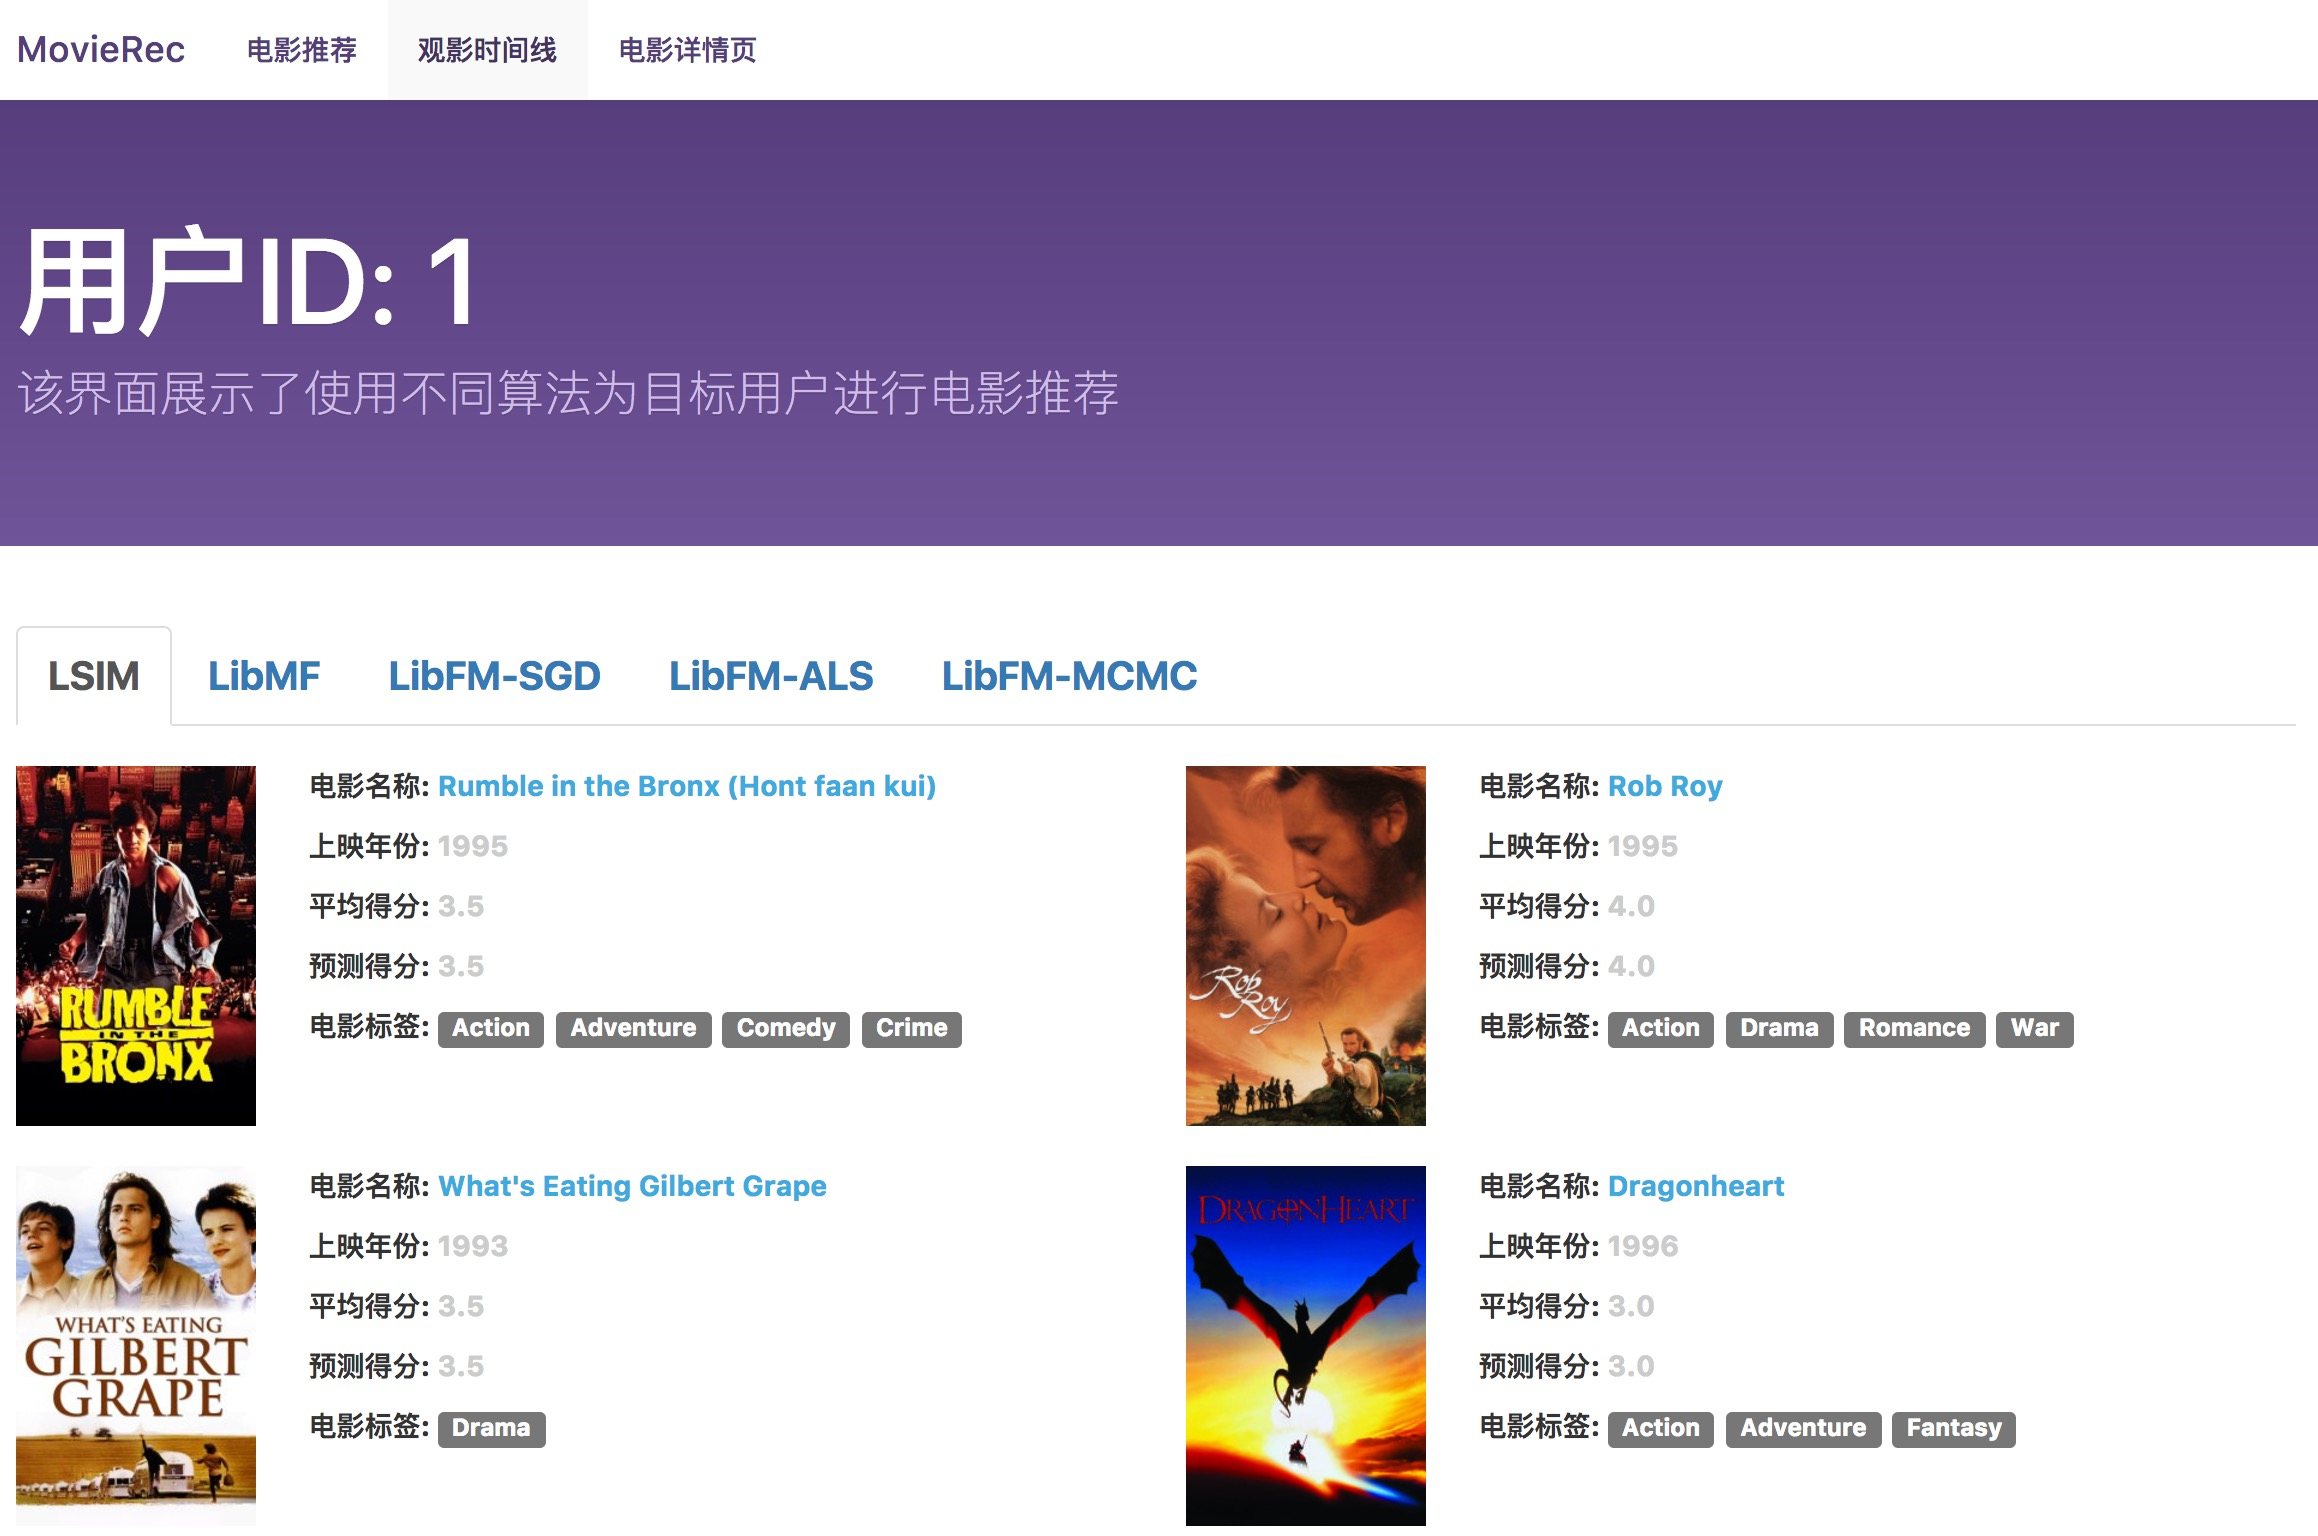
\includegraphics[scale=0.16]{images/systemshow1.jpeg}
\caption{MoiveRec中的电影推荐界面}
\label{fig:systemshow1}
\end{figure}

电影推荐界面作为整个推荐系统的核心,是所有界面中最重要的一个,图\ref{fig:systemshow1}展示了MovieRec中的电影推荐界面。
从图中可以看出,MovieRec中实现了本文中提出的多层感知器模型和长短期兴趣模型,在图中分别以UM、U-M以及LSIM进行表示,
同时实现了经典的基于矩阵分解和因式分解机的推荐算法,在图中分别以LibMF、LibFM-SGD、LibFM-ALS以及LibFM-MCMC进行表示,
用户可以通过点击导航栏在不同的推荐算法中进行切换,选择自己满意的推荐结果。
每个推荐列表一共包含$20$部电影,每项推荐电影提供了对应的电影海报和电影名称信息,用户可以通过点击它们跳转到对应的电影详情界面。
同时还提供了电影的平均评分和推荐算法的预测评分,目前推荐列表是使用预测评分进行排序的,另外一种可选方案是使用预测得分和评分得分的差值进行排序,
这样可以帮助用户发现大众不喜爱但是符合自己口味的小众电影。

\begin{figure}[htbp]
\centering
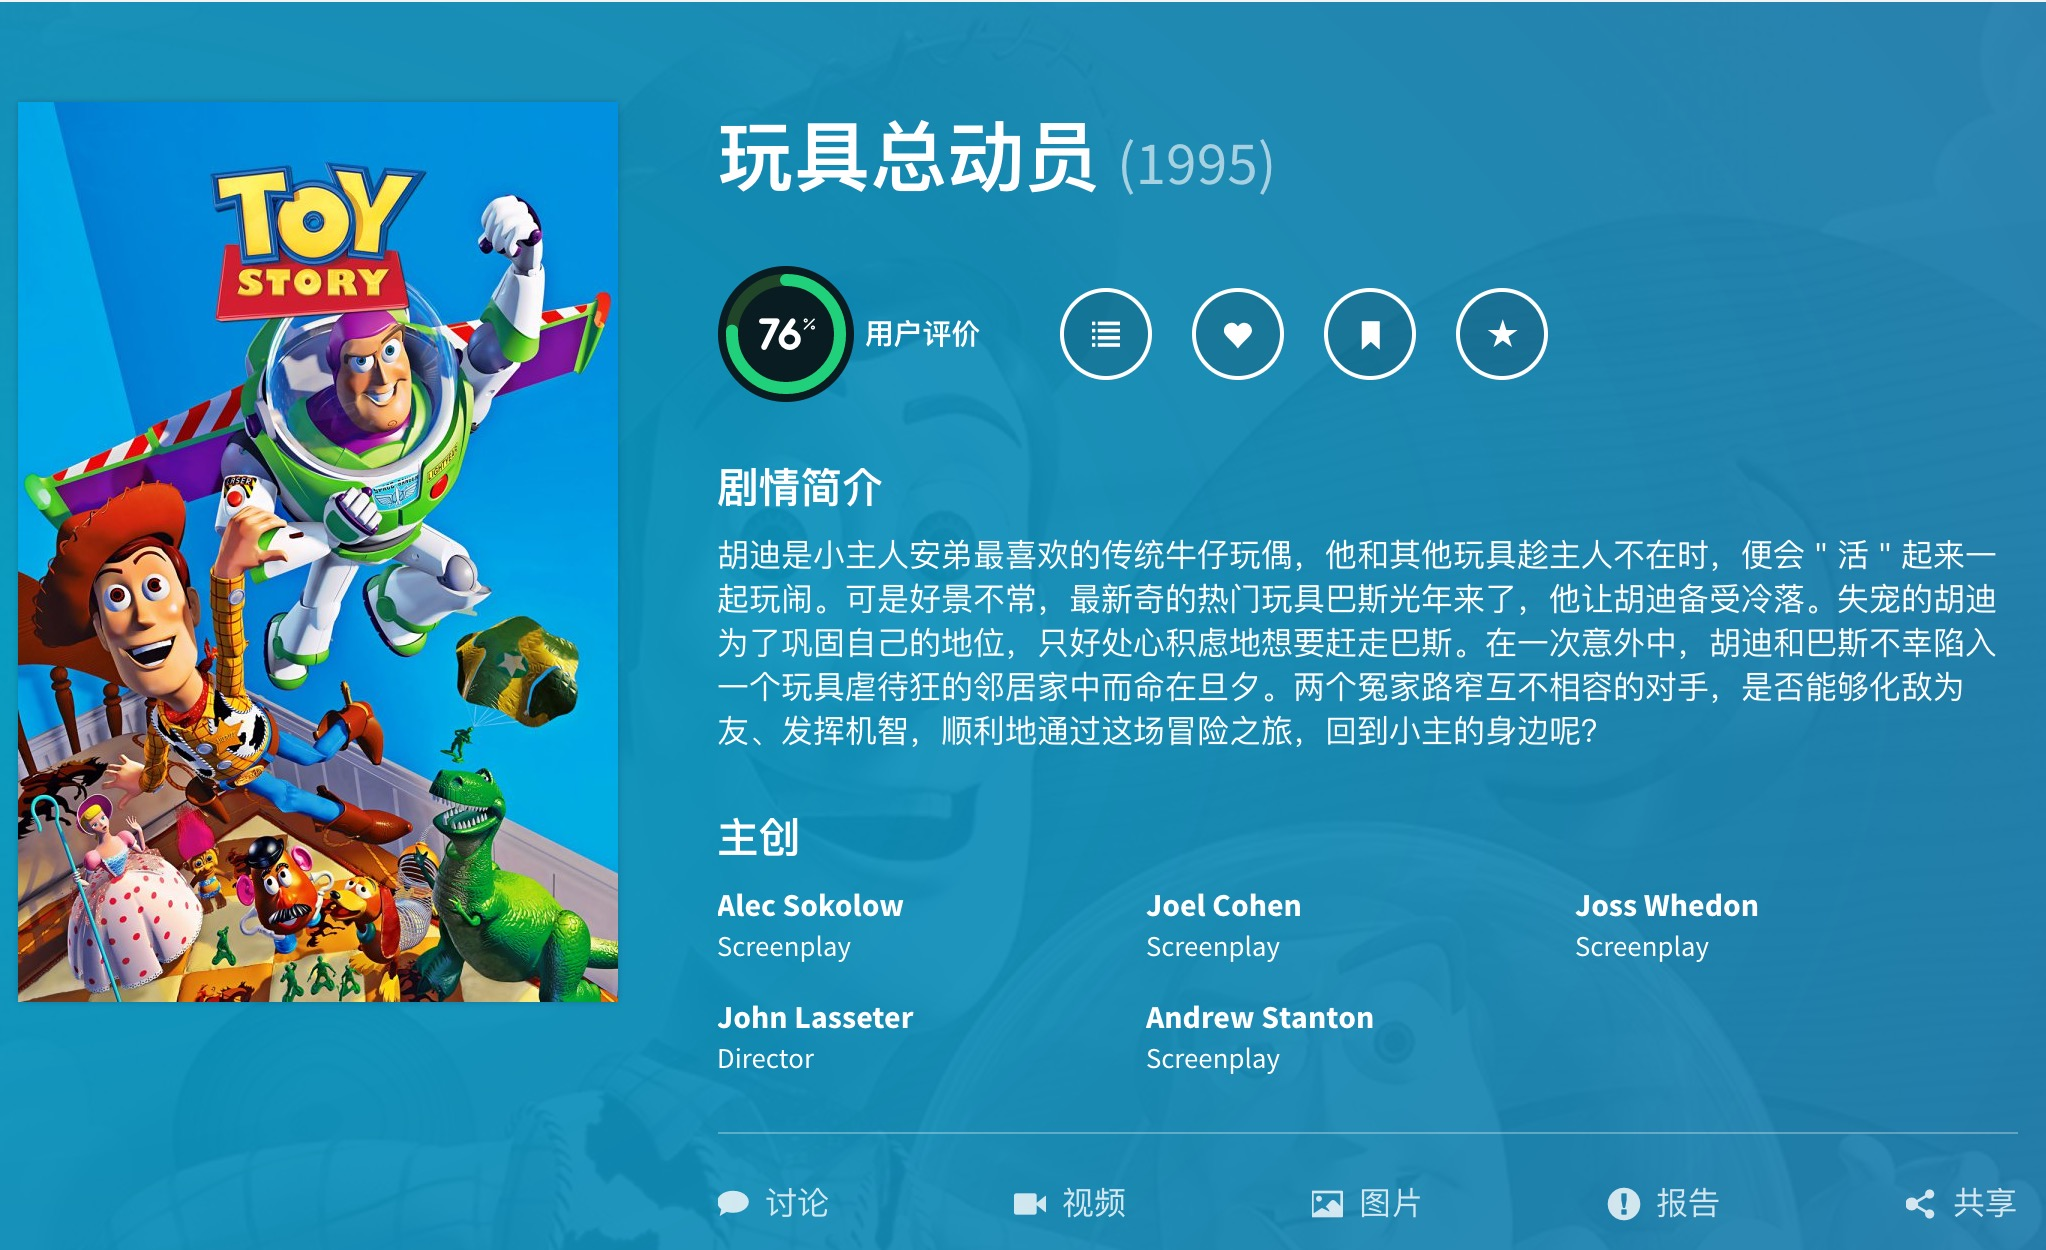
\includegraphics[scale=0.16]{images/systemshow2.jpeg}
\caption{MoiveRec中的观影时间线界面}
\label{fig:systemshow2}
\end{figure}

\begin{figure}[htbp]
\centering
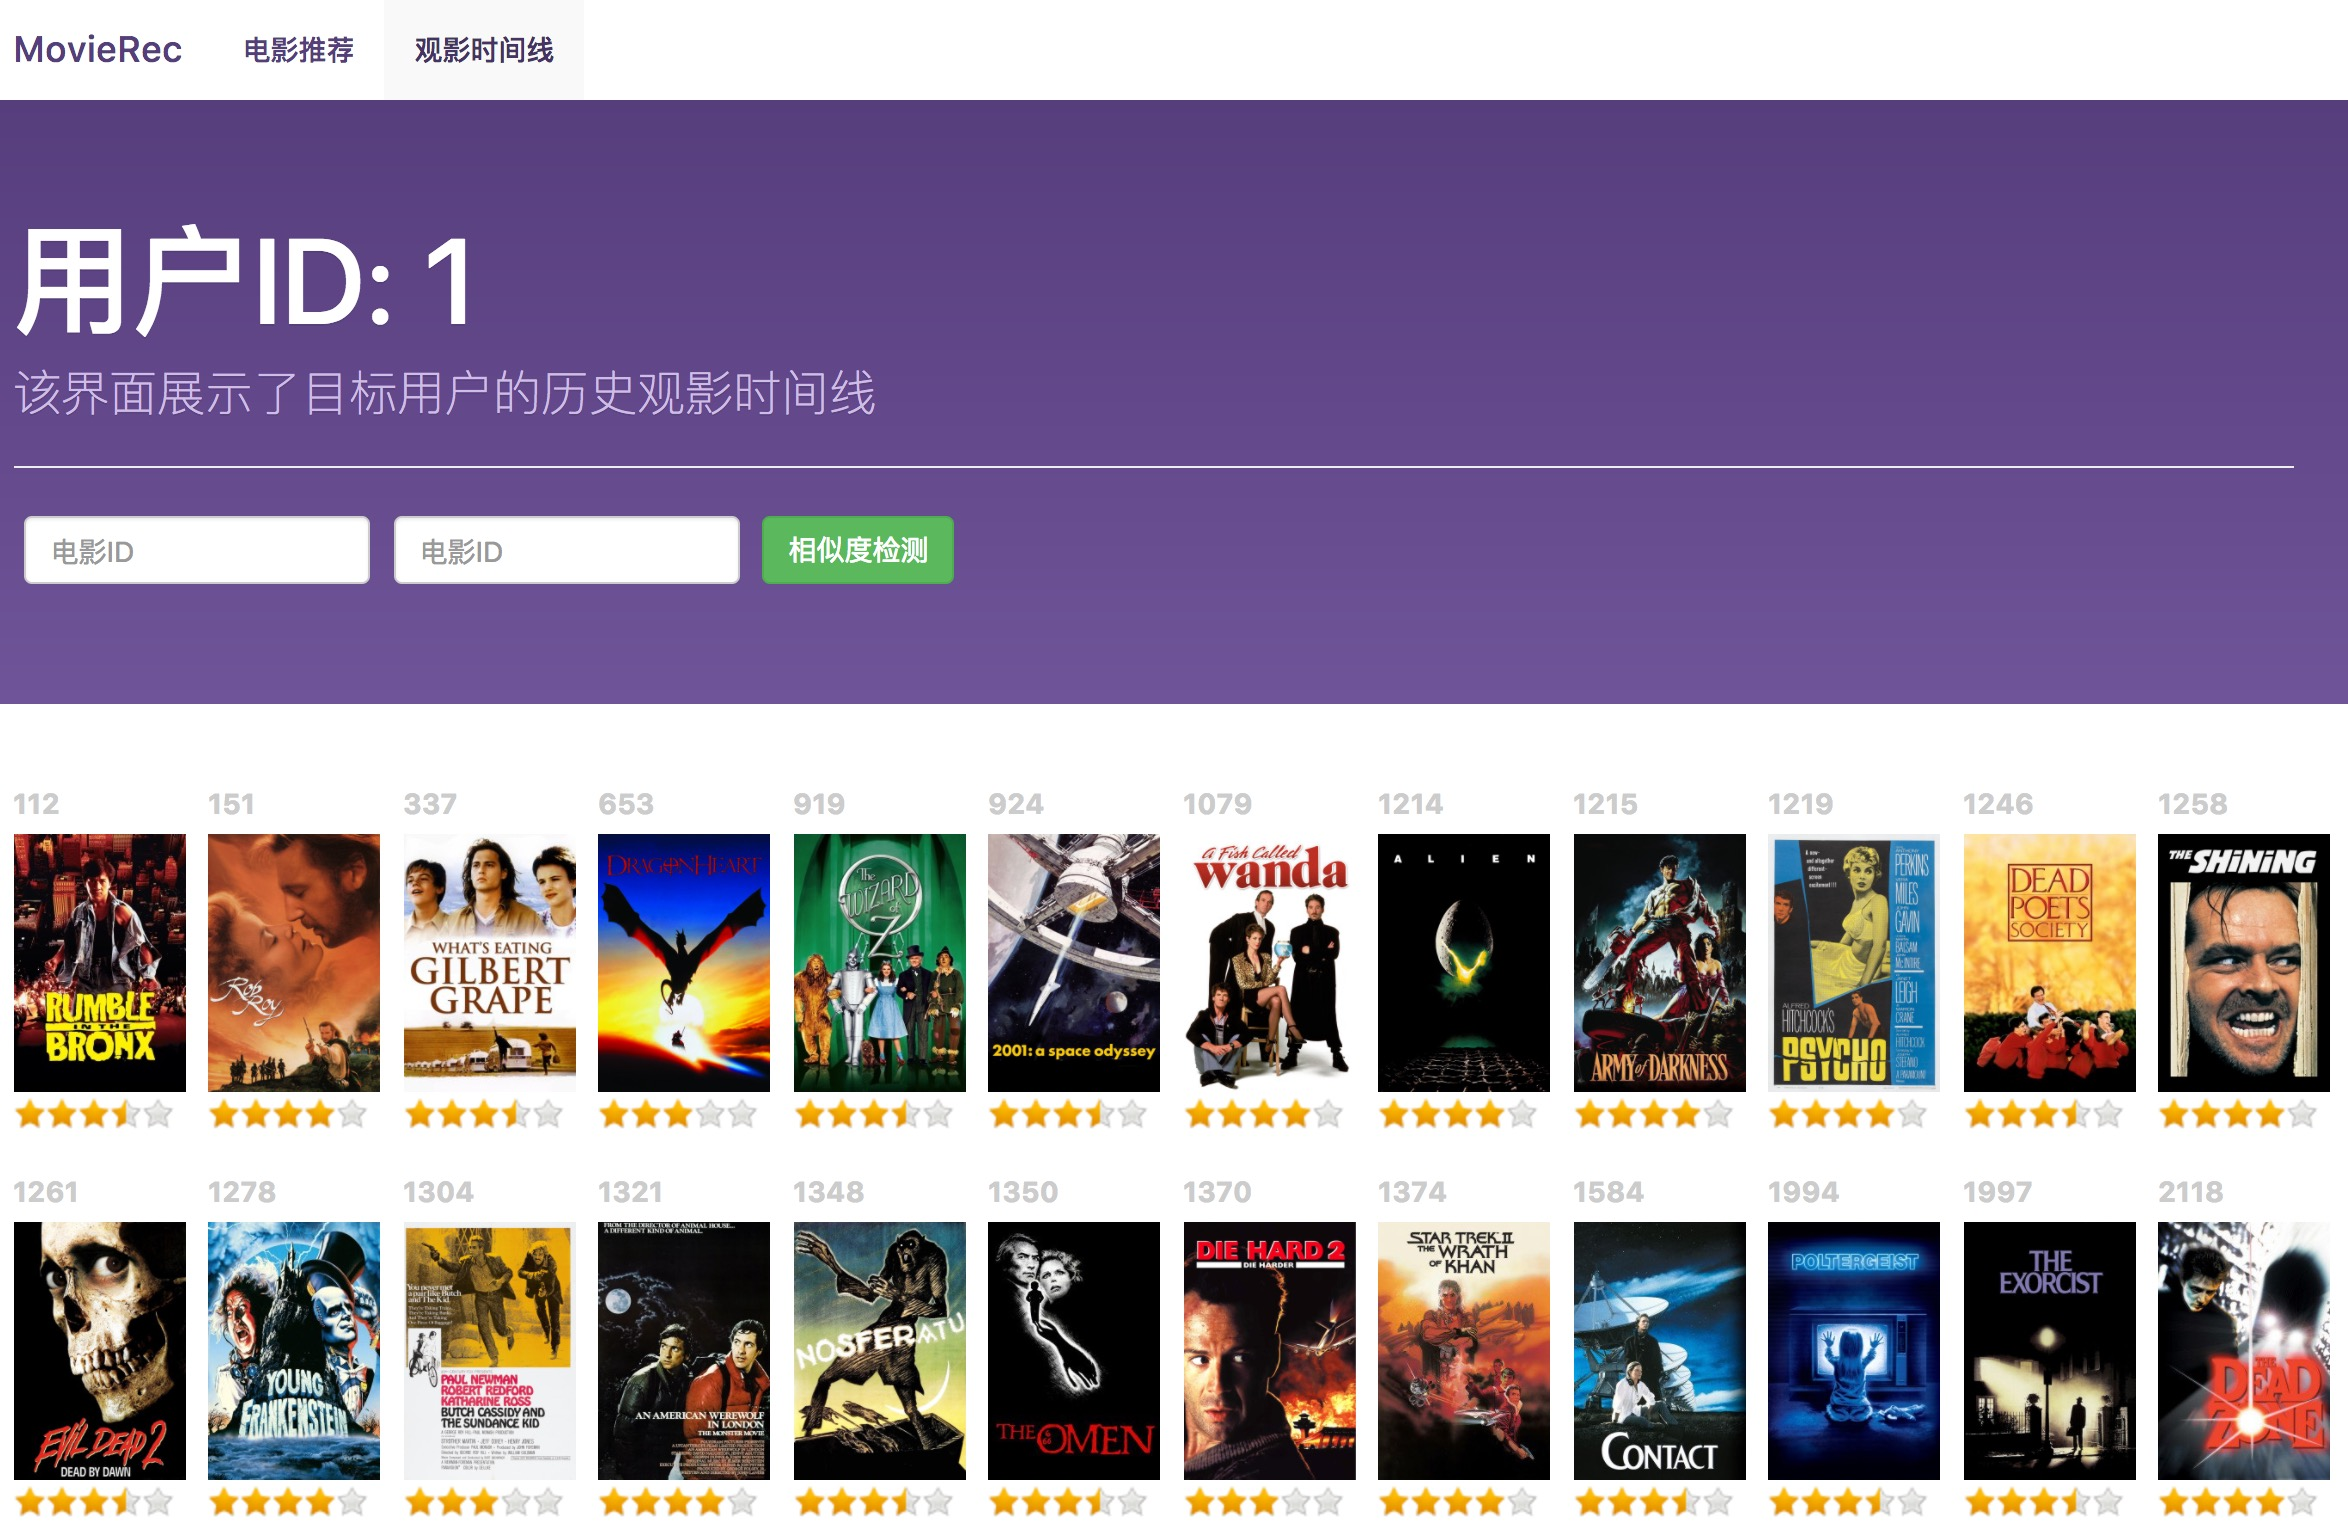
\includegraphics[scale=0.16]{images/systemshow3.jpeg}
\caption{MoiveRec中的电影详情界面}
\label{fig:systemshow3}
\end{figure}

特别地,针对本文提出的基于用户兴趣漂移的长短期兴趣模型,MovieRec还提供了用户的观影时间线界面,如图\ref{fig:systemshow2}所示。
在该界面中,我们标记出了目标用户历史上所有有过评分记录的电影,并按照评分时间进行了排序,排序列表中主要包含了电影ID、电影海报以及评分数据等信息,
用户可以通过点击电影ID或者电影海报跳转到对应的电影详情界面。
同时,在长短期兴趣模型中,我们生成了带时序特征的用户表示和电影表示,
还提出了同一个观影时间线上,相距较近的电影之间的相似度高于相距较远的电影的基础假设。
所以观影时间线界面上还提供了计算电影相似度接口,用户在蓝色区域输入想要对比的两部电影的ID信息,即可定性地对比两者之间的相似度。
另外,用户通过浏览时间线可以直观上得出长时间以来自己的观影兴趣转变。

电影详情界面可以帮助用户更好地了解一部电影的各个方面,除了刚刚提到的一些电影基本属性,电影详情界面还额外提供了电影的剧情简介、
电影的导演和主演信息,电影的社区评价等等。因为当前平台的用户数量较少,参与度也较低,所以MovieRec还额外索引了MovieLens、
IMDb和TMDb三个著名电影推荐平台上对应的电影详情界面,用户可以通过导航栏进行切换,查看在不同电影推荐平台上其他用户的评分和评论数据,
图\ref{fig:systemshow3}就展示了电影《Breaking the Waves》在MovieLens平台上的电影详情页面。


